\documentclass[12pt]{article} 

\usepackage{amsmath,amsthm,amssymb,hyperref}
\usepackage{geometry}
\usepackage{verbatim}
\usepackage{minted}
\usepackage{graphicx}
\setminted{
  fontsize=\small,
  linenos,
  breaklines,
  frame=lines,
  bgcolor=codebg,
  style=friendly
}

\usepackage{xcolor}
\definecolor{codebg}{HTML}{F7F7F7}

\setlength{\parindent}{0pt}
\setlength{\parskip}{0.6em}

\hypersetup{
    colorlinks=true,
    linkcolor=blue}
    
\newtheorem*{theorem}{Theorem}
\newtheorem*{conjecture}{Conjecture}
\newtheorem*{lemma`}{Lemma}
\newtheorem*{corollary}{Corollary}
\newtheorem*{proposition}{Proposition}

\theoremstyle{definition}
\newtheorem*{defn}{Definition}

\newcommand{\N}{\mathbb{N}}
\newcommand{\Z}{\mathbb{Z}}
\newcommand{\R}{\mathbb{R}}
\newcommand{\Q}{\mathbb{Q}}
\newcommand{\term}[1]{\texttt{"#1"}}
\newcommand{\nt}[1]{\text{#1}}

% --- Main Document Body ---
\begin{document}
    \noindent
    Rhys Wiers\\
    CIS 343\\
    Dr. Haoyu Li\\
    \today

    \begin{center}
        {\Large \textbf{Lab 3: Parser}}
    \end{center}

    \begin{enumerate}
    \item \textbf{Grammar:}
        \begin{equation*}
        \begin{array}{lcl}
        \nt{expression} & \rightarrow & \nt{logic\_or} \\[4pt]
        \nt{logic\_or}  & \rightarrow & \nt{logic\_and}\ \left(\,\term{\textbar\textbar}\ \nt{logic\_and}\,\right)* \\[4pt]
        \nt{logic\_and} & \rightarrow & \nt{equality}\ \left(\,\term{\&\&}\ \nt{equality}\,\right)* \\[4pt]
        \nt{equality}   & \rightarrow & \nt{comparison}\ \left(\,(\term{!=} \mid \term{==})\ \nt{comparison}\,\right)* \\[4pt]
        \nt{comparison} & \rightarrow & \nt{term}\ \left(\,(\term{>} \mid \term{>=} \mid \term{<} \mid \term{<=})\ \nt{term}\,\right)* \\[4pt]
        \nt{term}       & \rightarrow & \nt{factor}\ \left(\,(\term{-} \mid \term{+})\ \nt{factor}\,\right)* \\[4pt]
        \nt{factor}     & \rightarrow & \nt{unary}\ \left(\,(\term{/} \mid \term{*} \mid \term{\%})\ \nt{unary}\,\right)* \\[4pt]
        \nt{unary}      & \rightarrow & (\term{!} \mid \term{-})\ \nt{unary} \mid \nt{primary} \\[4pt]
        \nt{primary}    & \rightarrow & \texttt{NUMBER} \mid \texttt{STRING} \mid \term{true} \mid \term{false} \mid \term{nil} \\
                        &             & \mid\ \term{(}\ \nt{expression}\ \term{)}
        \end{array}
        \end{equation*}

    \item \textbf{Associativity}
        All grammar rules are left associativy with the exception of the unary operators.

    \item \textbf{Test Cases}
        From the project root, you can run the following to compile and run the parser tests:
        \begin{minted}{bash}
g++ -std=c++17 -Isrc test/lab3/parser-test.cpp $(ls src/*.cpp | \
grep -v main.cpp) -o parser-test
        \end{minted}
        Then run the executable:
        \begin{minted}{bash}
./parser-test
        \end{minted}

        The following is the output I got of the test cases. It covers all grammar rules that the parser handles.
        \begin{minted}{bash}
ok   number
ok   decimal
ok   string
ok   true
ok   false
ok   nil
ok   unary minus
ok   unary bang
ok   nested bang
ok   nested minus
ok   group
ok   nested group
ok   factor over term
ok   term after factor
ok   group overrides
ok   unary over factor
ok   unary over equality
ok   term over comparison
ok   comparison over equality
ok   and over or
ok   and before or
ok   remainder is factor
ok   assignment example
ok   minus
ok   slash
ok   equality
ok   or
ok   binary then unary
ok   full
ok   logic
[line 1] Error at end: Expected expression.
ok   empty input
[line 1] Error at end: Expected expression.
ok   trailing operator
[line 1] Error at '*': Expected expression.
ok   leading operator
[line 1] Error at '+': Expected expression.
ok   double operator
[line 1] Error at end: Expected ')' after expression.
ok   missing close paren
[line 1] Error at ')': Expected expression.
ok   empty group
[line 1] Error at ')': Expected expression.
ok   lone close paren
[line 1] Error at '2': Expected end of expression.
ok   trailing token

All tests passed.
        \end{minted}

        The errors are caused by:
        \begin{enumerate}
            \item Empty input
            \item ``+" with nothing after
            \item Two ``+" in a row
            \item No closing parenthesis after an opening one earlier in the expression
            \item Empty parentheses
            \item Two numbers with nothing in between
        \end{enumerate}
    
        \newpage
    \item \textbf {Example AST}

        Here is the tree for ``1 + 2 * 3":
        \begin{figure}[htbp]
          \centering
          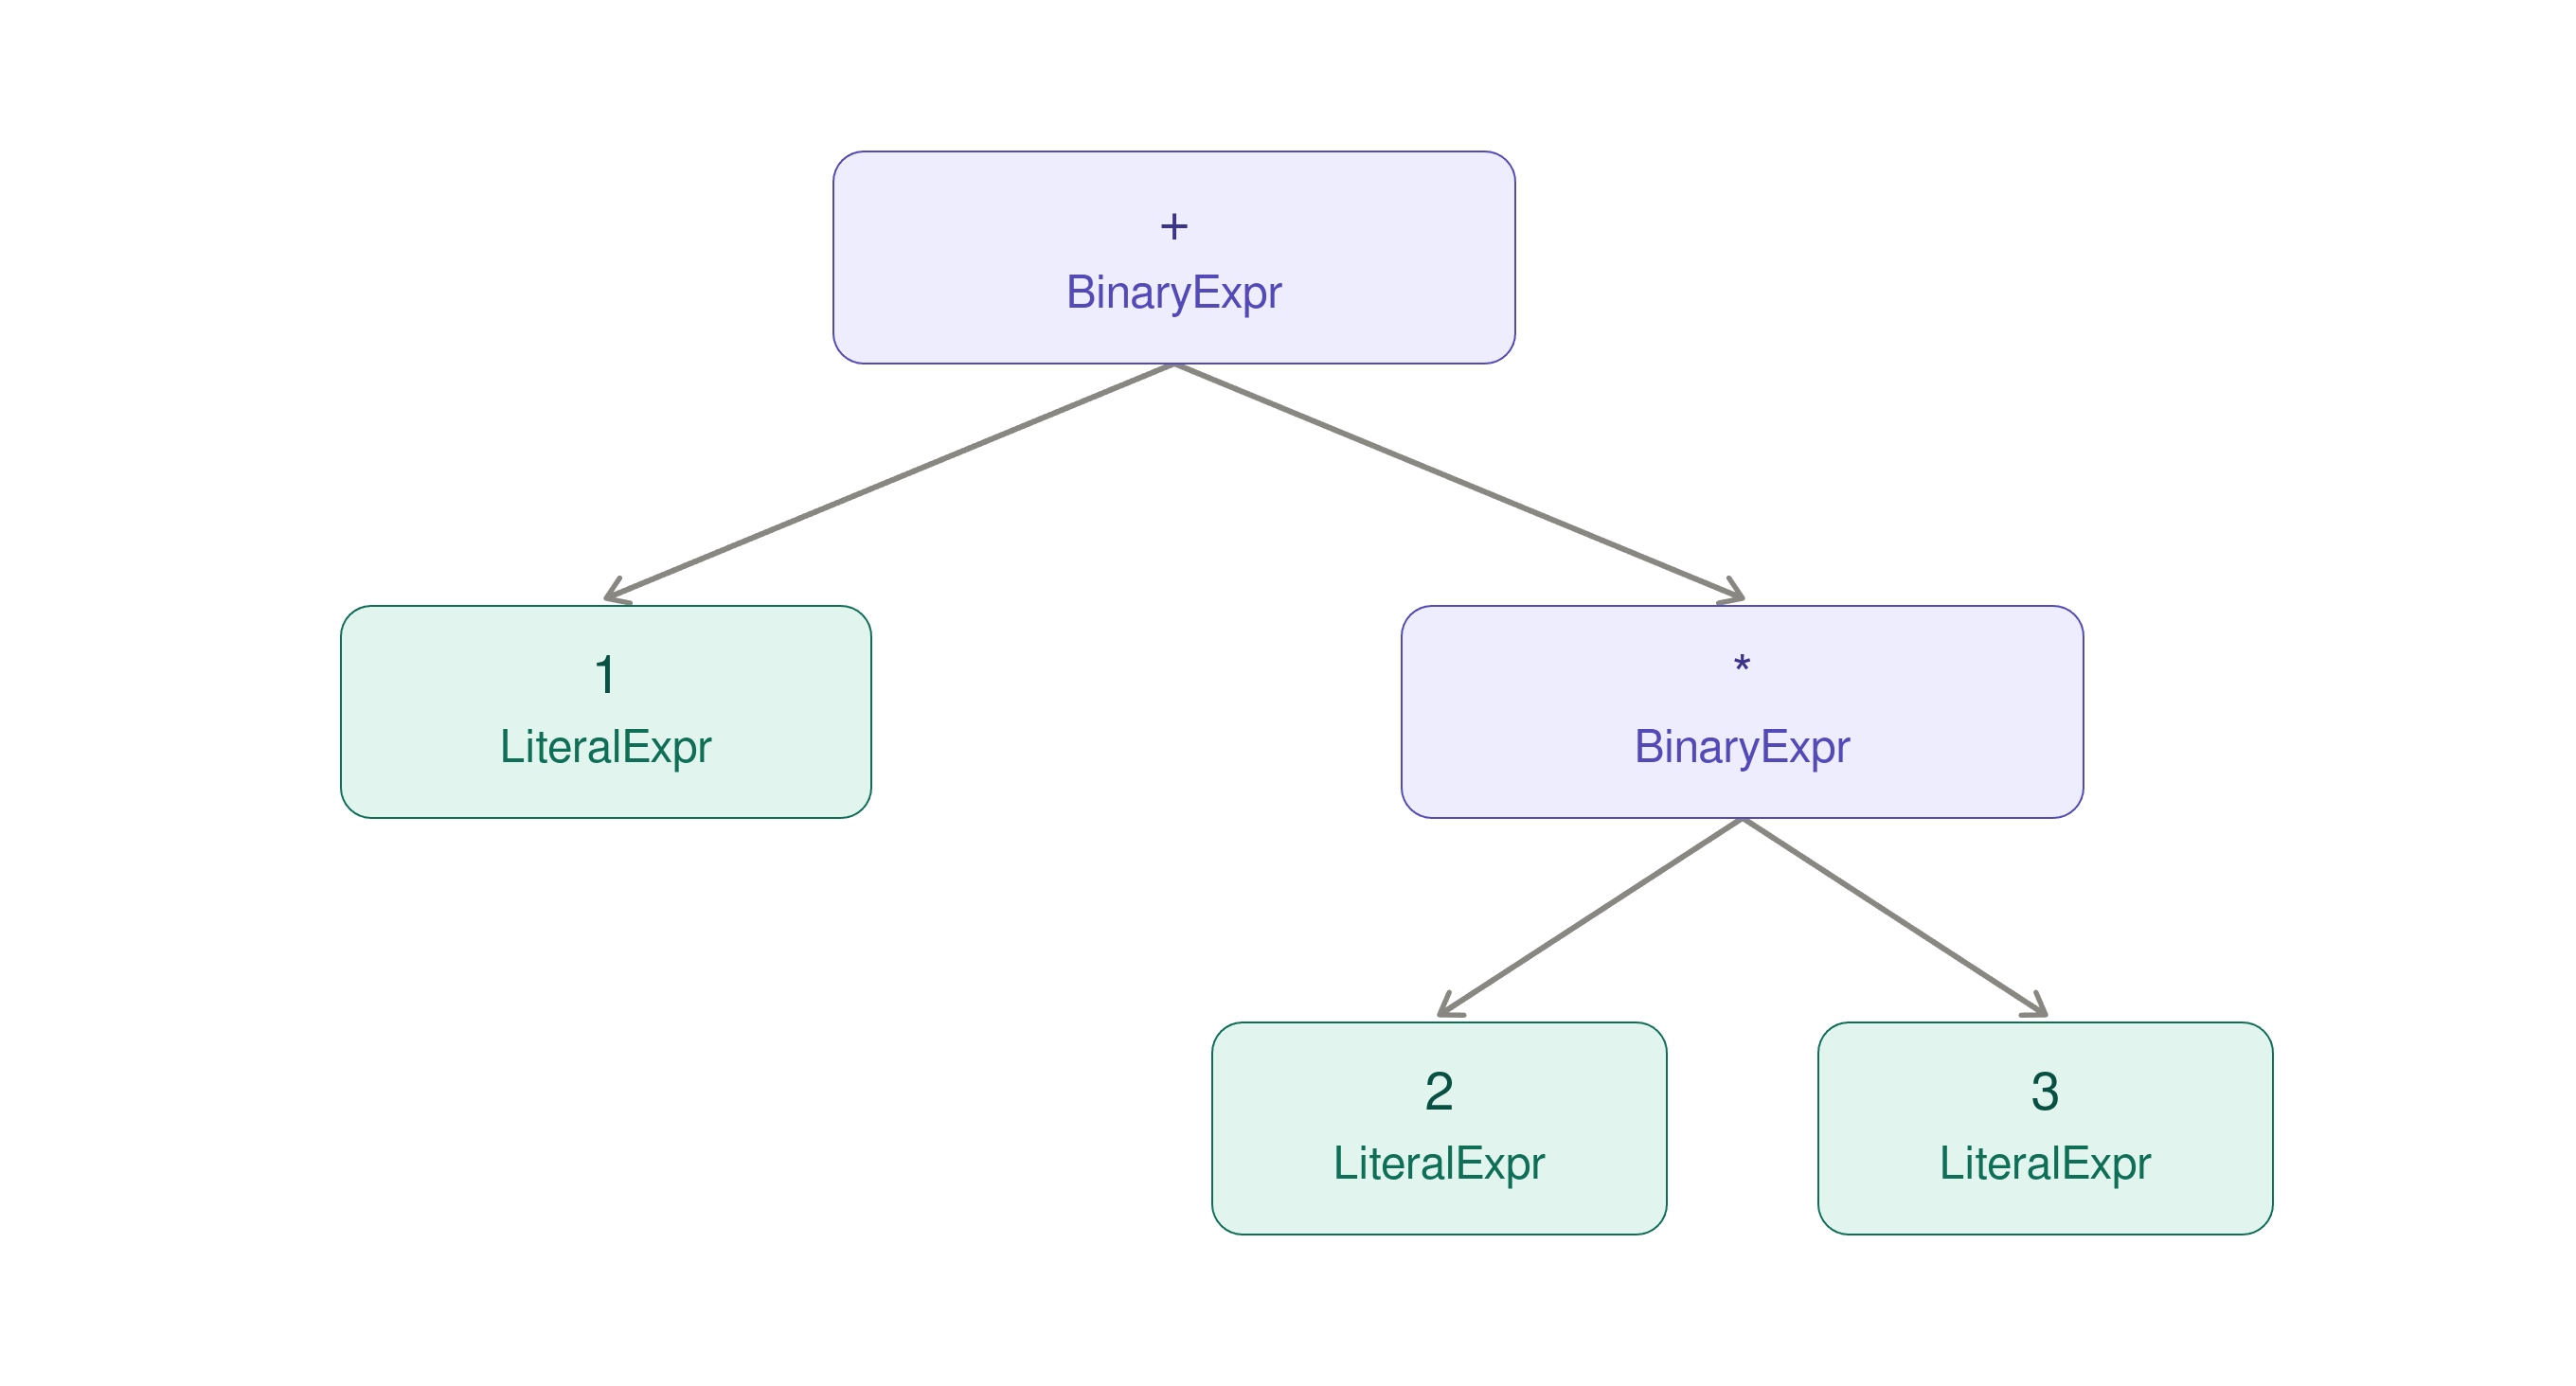
\includegraphics[width=0.8\textwidth]{ast_for_1_plus_2_times_3.png}
          \label{fig:ast}
        \end{figure}
            
        The parser first reads 1 and holds onto it. Then it sees +, so it knows it needs something to add to 1, but before deciding what, it looks at what comes next. It reads 2 and then sees *. Multiplication has higher precedence than addition, so the 2 belongs with the 3, not with the 1. It bundles 2 * 3 together. Now it can finish the addition: 1 + (2 * 3).
        
        This results in the tree shown above.

\end{enumerate}
\end{document}
